% ----------------------------------------------------------------------
%  Základní nastavení dokumentu - musí být na začátku každého tex
%  (pořadí příkazů v této části je důležité!)
% ----------------------------------------------------------------------

%  Typ dokumentu - článek, prezentace aj.
% Standardní základ
%\documentclass[a4paper,10pt]{article} 
%\usepackage[letterpaper]{geometry}
%\geometry{verbose,tmargin=1.5cm,bmargin=2cm,lmargin=2cm,rmargin=2cm}

% Alternativní verze - vhodnější formát papíru (větší hustota textu)
%\documentclass[10pt]{scrartcl}
%\KOMAoptions{DIV=20} % formát papíru a odsazení od jeho okrajů
\documentclass{prepareprotokol} %všechny balíčky pro protokol + titulní strana

%  Kódování výstupu - aby šlo z pdf kopírovat včetně háčků a čárek
\usepackage[T1]{fontenc} 

%  Kódování vstupu - v kódu lze použít háčky a čárky
\usepackage[utf8]{inputenc} 

%  Základní typografická pravidla češtiny/slovenštiny
\usepackage[czech]{babel} 
%\usepackage[slovak]{babel}
% použijte jen jeden z příkazů


%  Lépe vypadající písmo pro T1 kódování
\usepackage{lmodern} 
% je možno zakomentovat, nepoužívá-li se T1 kódování




%  Formátování stránek, empty = odstraní číslování
% \pagestyle{empty}

%  Řádkování
\linespread{1.1}


% ----------------------------------------------------------------------
%  Doplňující balíčky
% ----------------------------------------------------------------------

%  Po desetinné čárce v matematickém módu se nevytvoří mezera
\usepackage{icomma} 

%  Umožňuje pracovat s grafikou
\usepackage{graphicx}

%  Umožňuje použít dva obrázky vedle sebe
\usepackage{subcaption}

%  Pro vkládání obrázků ve formátu eps (např. z gnuplot)
\usepackage{epstopdf} 

%  Automaticky odsadí i první paragraf v každé sekci
\usepackage{indentfirst}

%  Umožňuje rozdělovat obsah na více sloupců
\usepackage{multicol}
\usepackage{booktabs}
\usepackage{pgffor}

%  Umožňuje používat hypertextové odkazy, nastavuje jejich vlastnosti
\usepackage[unicode]{hyperref}


% ----------------------------------------------------------------------
%  Matematika
% ----------------------------------------------------------------------

%  Lepší zobrazování matematiky (rozšíření sum o \limits atd.)
\everymath{\displaystyle}

%  Široké spektrum příkazů pro matematiku
% (Umožní např. psát přes \mathbb{N/R/Q/..} množiny čísel)
\usepackage{amsmath,amssymb}

%  Velikost fontu matematických výrazů v dokumentu lze pro danou
% základního fontu dokumentu upravit pomocí:
% \DeclareMathSizes{X}{Y}{Z}{U} kde:
% X je velikost fontu v dokumentu, pro kterou se matematika upraví
% Y je standartní velikost fontu matematiky
% Z je velikost fontu zmenšených (vnořených výrazů)
% U je velikost fontu ještě více zmenšených (vnořených výrazů).
\DeclareMathSizes{10}{10}{8}{7}

%  Široké spektrum příkazů pro fyziku
\usepackage{physics}

%  Psaní SI jednotek
\usepackage{siunitx}

%  Nám bližší zápis písmene epsilon
\AtBeginDocument{%
%\let\phi\varphi
\let\epsilon\varepsilon
}


% ----------------------------------------------------------------------
%  Pro češtinu/slovenštinu
% ----------------------------------------------------------------------

%  Lokalizace některých názvů do češtiny/slovenštiny
\addto\captionsczech{\renewcommand{\figurename}{Obr.}}
\addto\captionsczech{\renewcommand{\tablename}{Tab.}}
%\addto\captionsczech{\renewcommand{\refname}{Reference}}

\addto\captionsslovak{\renewcommand{\figurename}{Obr.}}
\addto\captionsslovak{\renewcommand{\tablename}{Tab.}}
%\addto\captionsslovak{\renewcommand{\refname}{Reference}}

% Odkomentujte následující příkaz, máte-li stažený balíček encxvlna 
% (nutno stáhnout manuálně)
%\usepackage{encxvlna} %vloží nezlomitelné mezery k jednopísmenným



% ----------------------------------------------------------------------
%  Soubor s makry
% ----------------------------------------------------------------------
%% ----------------------------------------------------------------------
%  Identifikace protokolu (příkazy lze použít v celém dokumentu)
% ----------------------------------------------------------------------

%  Nastaví autora, název, datum, skupinu měření apod. 
\newcommand{\Institute}{FJFI~ČVUT~v~Praze}
%\newcommand{\Subject}{Základy fyzikálních měření}
\newcommand{\Subject}{Fyzikální praktikum II}  %odkomentujte dle potřeby

%  Máte-li více spoluměřících než jednoho, vložte jen jejich příjmení
\newcommand{\Author}{Jméno autora}
\newcommand{\Coauthor}{Jméno kolegy} 
\newcommand{\Group}{Pátek} %den, kdy chodíte na praktika, nikoli obor
\newcommand{\Circle}{2} %číslo skupiny v rámci praktika, nikoli kruh

%  Tato část bude v každém protokolu jiná, nezapomeňte upravit!
\newcommand{\Title}{Úloha 0 -- Psaní vzorového protokolu}
\newcommand{\Labdate}{1.1.2017} %datum měření, nikoli datum odevzdání
\newcommand{\Worktime}{5 h} %jak dlouho vám trvalo vypracování protokolu




% ----------------------------------------------------------------------
%  Vlastní příkazy
% ----------------------------------------------------------------------


%  Matematika
\newcommand{\ee}{\mathrm{e}} %eulerovo číslo
\newcommand{\ii}{\mathrm{i}} %imaginární jednotka

% Jednotky
%\newcommand{\unit}[1]{\,\mathrm{#1}} %jednotky zadávejte pomocí tohoto příkazu
\renewcommand{\deg}{\ensuremath{\mathring{\;}}} %symbol stupně
\newcommand{\celsius}{\ensuremath{\deg\mathrm{C}}} %stupně celsia

%(hodnota plus mínus chyba) jednotka
\newcommand{\hodn}[3]{(#1 \pm #2)\unit{#3}} 

%veličina [jednotka] do hlavičky tabulky
\newcommand{\tabh}[2]{\ensuremath{#1\,[\mathrm{#2}]}} 


% ----------------------------------------------------------------------
%  Vlastní příkazy
% ----------------------------------------------------------------------


%  Matematika
\newcommand{\ee}{\mathrm{e}} %eulerovo číslo
\newcommand{\ii}{\mathrm{i}} %imaginární jednotka

% Jednotky
%\newcommand{\unit}[1]{\,\mathrm{#1}} %jednotky zadávejte pomocí tohoto příkazu
\renewcommand{\deg}{\ensuremath{\mathring{\;}}} %symbol stupně
\newcommand{\celsius}{\ensuremath{\deg\mathrm{C}}} %stupně celsia

%(hodnota plus mínus chyba) jednotka
\newcommand{\hodn}[3]{(#1 \pm #2)\unit{#3}} 

%veličina [jednotka] do hlavičky tabulky
\newcommand{\tabh}[2]{\ensuremath{#1\,[\mathrm{#2}]}}

%  nachází se ve složce /tex/



% ----------------------------------------------------------------------
%  Nastavení odkazů a výsledného pdf
% ----------------------------------------------------------------------
\hypersetup{
colorlinks=true, 
citecolor=blue, 
filecolor=blue, 
linkcolor=blue,
urlcolor=blue, 
%pdftitle={\title},    % title
pdfauthor={Jonáš Venc},     % author
pdfsubject={Protokol},   % subject of the document
pdfcreator={Jonáš Venc},   % creator of the document
%     pdfproducer={Producer}, % producer of the document
%     pdfkeywords={keywords}, % list of keywords
pdfnewwindow=true,      % links in new window
}

% ----------------------------------------------------------------------
%  Začátek dokumentu - formátování na výstup
% ----------------------------------------------------------------------

\praktikum{I} %číslo praktika (I, II nebo III)
\autor{Jonáš Venc} %jméno autora
\datum{4.\,3.\,2024} %datum měření
\cislo{27} %číslo úlohy
\nazev{Tepelné čerpadlo} %název úlohy

\begin{document}

\maketitle

% ----------------------------------------------------------------------
%  Tělo dokumentu
% ----------------------------------------------------------------------

\setlength{\parindent}{0.5cm}

% ----------------------------------------------------------------------
%  Protokol

\pagenumbering{arabic}  % číslování stránek čísly
% ----------------------------------------------------------------------
%  Pracovní úkoly
% ----------------------------------------------------------------------
\section{Pracovní úkoly}

\begin{enumerate}
\item Experimentálně ověřte platnost vztahu pro časovou závislost středního kvadratického posunutí částice \(\overline{s^2}\) při Brownově pohybu.

\item Určete aktivitu Brownova pohybu \(A\) submikronových částic ve vodě za pokojové teploty.

\item Velikost částic odečtěte z fotografie pomocí programu Solarius.

\item Vypočtěte Avogadrovu konstantu \(N_A\).

\end{enumerate}

% ----------------------------------------------------------------------
%  Teoretická část
% ----------------------------------------------------------------------
\section{Teoretická část}

Částice rozptýlené v plynu nebo v kapalině konají neustále náhodný, chaotický pohyb. Tento pohyb se nazývá Brownův pohyb. Je způsoben tepelnými fluktuacemi prostředí.

Pro popis pohybu částice se zavadí střední kvadratické posunutí \(\overline{x^2}\), jak je popsáno v [1], pro kterou platí vztah

\begin{equation}
    \overline{x^2} = A \cdot t
\end{equation}

kde \(A\) je aktivita Brownova pohybu a \(t\) čas.

Konstanta \(A\) lze pro kulovou částici vyjádřit jako

\begin{equation}
    A = \frac{R T}{3 \pi \eta r N_A}
\end{equation}

kde \(R\) je molární plynová konstanta, \(T\) teplota, \(\eta\) dynamická viskozita, \(r\) poloměr částice a \(N_A\) Avogadrova konstanta.

Pokud se budeme zabývat pohybem v rovině, nikoliv po jedno dimenzionální úsečce, rovnice pro střední kvadratické posunutí tvar

\begin{equation}
    \overline{s^2} = 2 \cdot A \cdot t
\end{equation}

Výpočet \(\overline{s^2}\) provádíme pomocí programu Brown, který vypočítá aritmetický průměr kvadrátu vzdáleností posunutí částice za časový interval.

Pokud označíme vzdálenost sousedních bodů jako \(s_t\) a vzdálenost bodů \(i\) a \(i + 2\) jako \(s_{2t}\) a analogicky \(s_{3t}\), poté podle rovnice (1) dostáváme

\begin{equation}
    \overline{s^2_{t}} \setminus \overline{s^2_{2t}} \setminus \overline{s^2_{3t}} = t \setminus 2t \setminus 3t
\end{equation}

Tento poměr můžeme později využít pro ověření kvality měření.

Viskozitu vzorku můžeme vyjádřit pomocí relativní viskozity \(\eta_{rel}\) jako

\begin{equation}
    \eta_{rel} = 1 + 2,5\varphi
\end{equation}

% ----------------------------------------------------------------------
%  Výsledky a zpracování měření
% ----------------------------------------------------------------------
\section{Výsledky a zpracování měření}

\subsection{Laboratorní podmínky}

    Měření bylo prováděno za laboratorních podmínek uvedených v tabulce \ref{tab:lab_pod}. Pro naše měření je ale důležitá teplota vzorku, která se nemusí přímo shodovat s teplotou vzduchu. Proto při práci s touto teplotou počítáme s větší chybou.

    \begin{table}[h]
        \centering
        \begin{tabular}{|c|c|c|} 
        \hline
            t / °C & p / hPa & vlhkost / \%RH  \\ 
        \hline
            23,4(4)   & 968,8(20)   & 31,0(25)            \\
        \hline
        \end{tabular}
        \caption{Laboratorní podmínky}
        \label{tab:lab_pod}
    \end{table}

Pro molární plynovou konstantu uvažujeme \(R\) = 8,314 $J$ ${mol}^{-1}$ $K^{-1}$.

\subsection{Časová závislost středního kvadratického posunutí}

Chování částic jsme sledovali pomocí optického mikroskopu, který měl výstup obrazu do počítače. Zde jsme díky programu Brown zaznamenávali jednotlivé polohy částic po časovém intervalu, který byl dán pravidelným zvukový signálem. Program bylo třeba nejprve kalibrovat, jak je popsáno v návodu u mikroskopu a ve studijním textu [1].

Vzorek byl umístěn na podlažní sklo mezi dvě krycí sklíčka a následně přikryt třetím krycím sklíčkem. Pro každou částici bylo třeba zaznamenat alespoň 25 poloh pro vyhodnocení výsledků. Časový interval byl nastaven na \(t\) = 5 s. Občas se stalo, že částice opustila sledovanou plochu, proto zde bylo měření ukončeno, nebo v případě zaznamenaných méně než 25 poloh bylo měřeni provedeno znovu.

Program Brown na konci měření vrátil naměřené hodnoty včetně vypočtených středních kvadratických posunutí. Pro vyhodnocení kvality měření byl použit teoretický vztah vztah (4). Celkově jsme změřili 9 částic a z nich jsme vybrali 6 nejkvalitnějších, jejichž výsledky jsou znázorněny v tabulce.

\begin{table}[h]
\centering
\begin{tabular}{|c|c|c|c|c|c|c|}
\hline
Číslo & Počet poloh & Poměry posunutí                    & I / s & \sigma_t / s & \overline{s^2} / \mu m^2 & A / \mu m^2 s^{-1} \\ \hline
3            & 25          & 1 : 1,63(40) : 2,53(59) : 3,50(82) & 5,00(1)              & 0,08                                        & 19,5(29)                                                                  & 1,95(4)                                                                                     \\
4            & 35          & 1 : 1,97(41) : 2,88(67) : 4,3(10)  & 5,00(1)              & 0,07                                        & 16,6(23)                                                                  & 1,66(3)                                                                                     \\
5            & 36          & 1 : 2,07(43) : 2,80(67) : 3,72(84) & 5,00(1)              & 0,13                                        & 23,4(31)                                                                  & 2,34(7)                                                                                     \\
7            & 52          & 1 : 2,24(53) : 3,14(76) : 4,4(11)  & 5,00(1)              & 0,14                                        & 17,9(29)                                                                  & 1,79(6)                                                                                     \\
8            & 25          & 1 : 2,12(62) : 3,1(10) : 4,1(12)   & 4,99(1)              & 0,13                                        & 17,7(30)                                                                  & 1,77(6)                                                                                     \\
9            & 59          & 1 : 2,02(49) : 3,28(74) : 4,31(96) & 5,00(1)              & 0,15                                        & 27,7(48)                                                                  & 2,8(1)                                                                                      \\ \hline
\end{tabular}
\caption{Měření pohybu sledovaných částic}
\label{tab:pohyb-castic}
\end{table}

kde $I$ je interval záznamu, \(\sigma_t\) Směrodatná odchylka jedné časové značky a $A$ je aktivita Brownova pohybu dopočtené z rovnice (3). Chyba aktivity Brownova pohybu je spočtena podle metody přenosu chyb [4] jako

\begin{equation}
    \sigma_A = A \sqrt{\frac{\sigma^2_{\overline{s^2}}}{\overline{s^2}} + \frac{\sigma^2_t}{t^2}}
\end{equation}

Vypočtené střední kvadratické posunutí i s jeho chybou jsme získali přímo z programu Brown.

Pro ověření lineární závislosti středního kvadratického posunutí na čase jsme tuto závislost měření číslo 8 znázornili na grafu \ref{fig:posunuti-na-case}. Tento graf jsme vytvořili v programu Origin a déle provedli lineární regresi. Bylo třeba započítat chybu ve směru osy Y a nastavit průsečík os s fitem na počátek.

\begin{figure}[h]
    \centering
    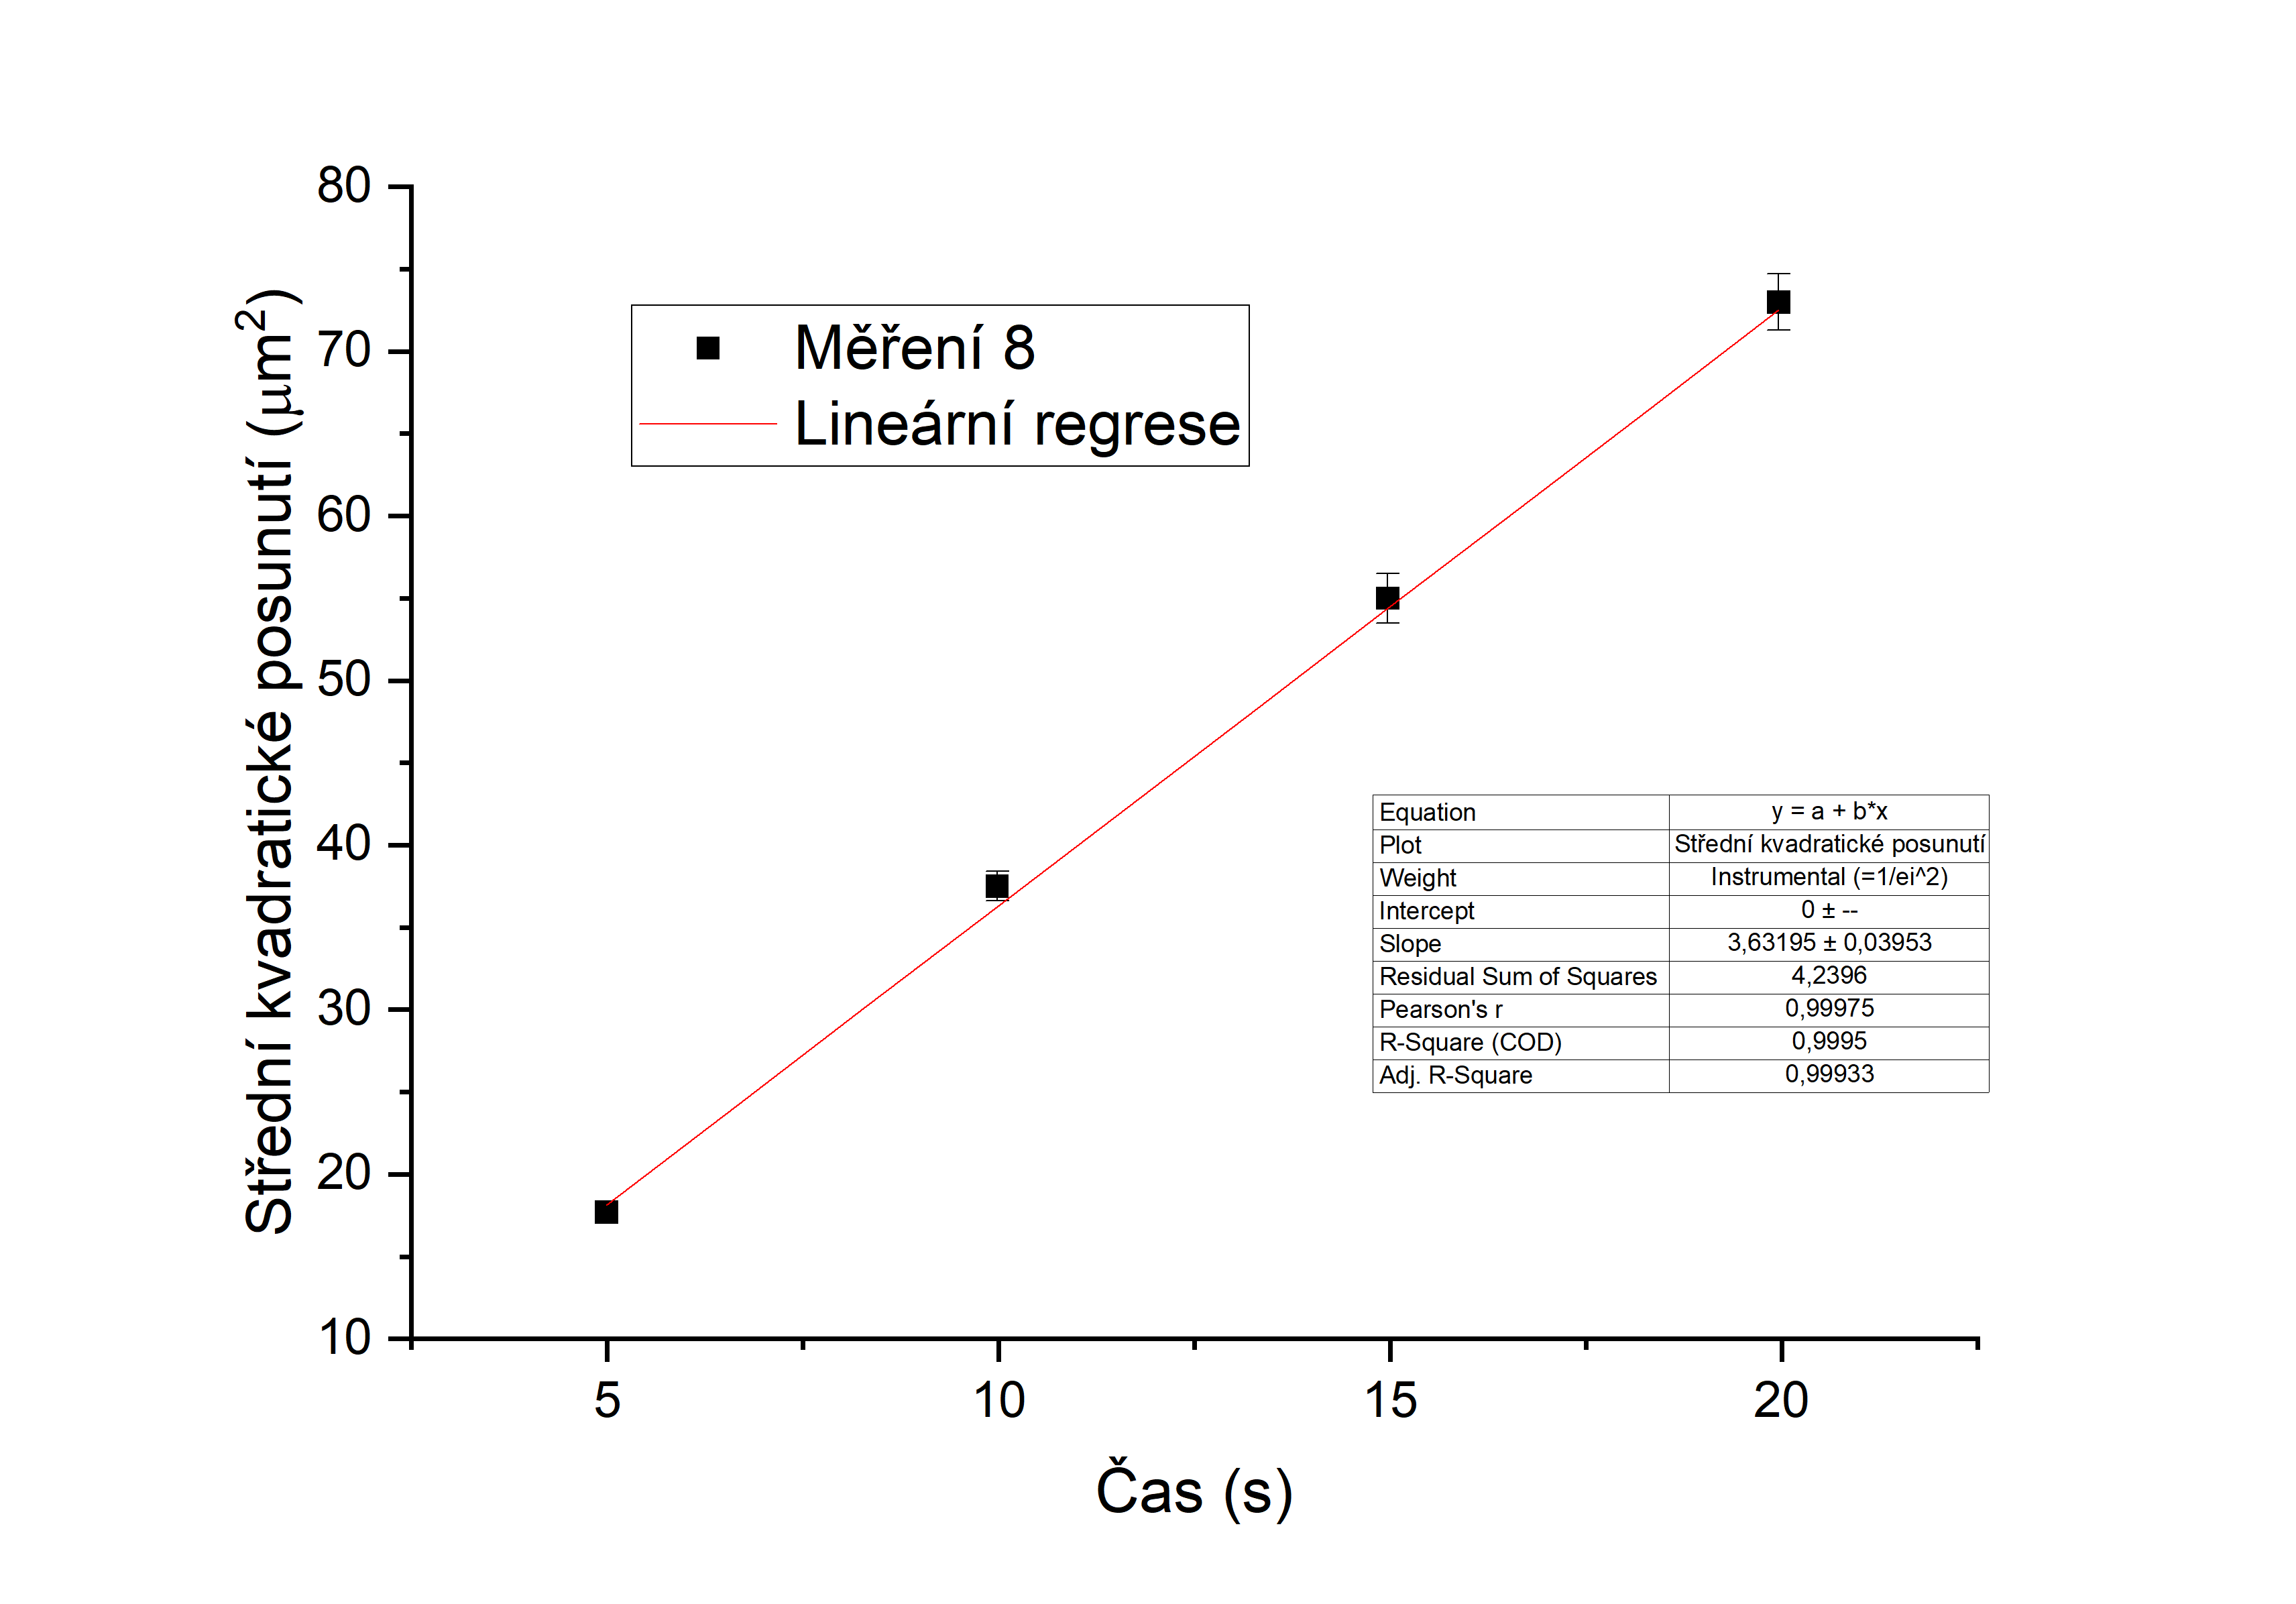
\includegraphics[width=0.85\linewidth]{16 - Brownův pohyb//Protokol - Brownův pohyb//img/Závislost posunutí na čase.png}
    \caption{Závislost středního kvadratického posunutí na čase}
    \label{fig:posunuti-na-case}
\end{figure}

\newpage
\subsection{Avogadrova konstanta}

Avogadrovu konstantu spočítáme podle rovnice (2). Jako teplotu použijeme teplotu vzduchu a započítáme větší nepřesnost, než by dovoloval teploměr. Déle budeme potřebovat dynamickou viskozitu vody. Ta byla stanovena podle tabulek při naší teplotě na hodnotu

\begin{equation}
    \nonumber
    \eta = 1 \cdot 10^{-3} \; Pa \cdot s
\end{equation}
    
% ----------------------------------------------------------------------
%  Diskuse výsledků
% ----------------------------------------------------------------------			
\section{Diskuse výsledků}

Intenzita pohybu - teplota a velikost molekuly.

Teplota vzorku - osvětlení.

Kalibrace i na konci měřen pro kontrolu.

Velikost kapky.

Utíkání částice a průběžné doostřování (3D pohyb).

Nekliknutí myši.

% ----------------------------------------------------------------------
%  Závěr
% ----------------------------------------------------------------------
\section{Závěr}

% ----------------------------------------------------------------------

% ----------------------------------------------------------------------
%  Literatura

\section{Použitá literatura}		
\begingroup
\renewcommand{\section}[2]{}
% ----------------------------------------------------------------------
%  Reference
% ----------------------------------------------------------------------

% sem doplňujte použité zdroje
\begin{thebibliography}{9}
\bibitem{bib:zadani} MFF. \emph{Studijní text:} [Online]. [cit. \today]. \newline \url{https://physics.mff.cuni.cz/vyuka/zfp/_media/zadani/texty/txt_103.pdf}

\bibitem{bib:tabulky} MIKULČÁK, Jiří; KLIMEŠ, Bohdan; ŠIROKÝ, Jaromír; ŠŮLA, Václav a ZEMÁNEK, František. \emph{Matematické, fyzikální a chemické tabulky pro střední školy.} 5. vydání. Pomocné knihy pro žáky (Prometheus). Praha: Prometheus, 2020. ISBN 978-80-7196-481-0. [cit. \today]

\end{thebibliography}

\endgroup
% ----------------------------------------------------------------------


% ----------------------------------------------------------------------
%  Příloha

% ----------------------------------------------------------------------

%\clearpage
				
%\clearpage


\end{document}

% ----------------------------------------------------------------------
%  Konec dokumentu
% ----------------------------------------------------------------------
